%!TEX program = xelatex

\documentclass[a4paper, openany, oneside]{memoir}
\usepackage[no-math]{fontspec}
\usepackage{pgfplots}
\pgfplotsset{compat=newest}
\usepackage{commath}
\usepackage{mathtools}
\usepackage{amssymb}
\usepackage{amsthm}
\usepackage{booktabs}
\usepackage{mathtools}
\usepackage{xcolor}
\usepackage[separate-uncertainty=true, per-mode=symbol]{siunitx}
\usepackage[noabbrev, capitalize]{cleveref}
\usepackage{listings}
\usepackage[american inductor, european resistor]{circuitikz}
\usepackage{amsmath}
\usepackage{amsfonts}
\usepackage{ifxetex}
\usepackage[dutch,english]{babel}
\usepackage[backend=bibtexu,texencoding=utf8,bibencoding=utf8,style=ieee,sortlocale=en_GB,language=auto]{biblatex}
\usepackage[strict,autostyle]{csquotes}
\usepackage{parskip}
\usepackage{import}
\usepackage{standalone}
\usepackage{hyperref}
%\usepackage[toc,title,titletoc]{appendix}

\ifxetex{} % Fonts laden in het geval dat je met Xetex compiled
    \usepackage{fontspec}
    \defaultfontfeatures{Ligatures=TeX} % To support LaTeX quoting style
    \setromanfont{Palatino Linotype} % Tover ergens in Font mapje in root.
    \setmonofont{Source Code Pro}
\else % Terug val in standaard pdflatex tool chain. Geen ondersteuning voor OTT fonts
    \usepackage[T1]{fontenc}
    \usepackage[utf8]{inputenc}
\fi
\newcommand{\references}[1]{\begin{flushright}{#1}\end{flushright}}
\renewcommand{\vec}[1]{\boldsymbol{\mathbf{#1}}}
\newcommand{\uvec}[1]{\boldsymbol{\hat{\vec{#1}}}}
\newcommand{\mat}[1]{\boldsymbol{\mathbf{#1}}}
\newcommand{\fasor}[1]{\boldsymbol{\tilde{\vec{#1}}}}
\newcommand{\cmplx}[0]{\mathrm{j}}
\renewcommand{\Re}[0]{\operatorname{Re}}
\newcommand{\Cov}{\operatorname{Cov}}
\newcommand{\Var}{\operatorname{Var}}
\newcommand{\proj}{\operatorname{proj}}
\newcommand{\Perp}{\operatorname{perp}}
\newcommand{\col}{\operatorname{col}}
\newcommand{\rect}{\operatorname{rect}}
\newcommand{\sinc}{\operatorname{sinc}}
\newcommand{\IT}{\operatorname{IT}}
\newcommand{\F}{\mathcal{F}}

\newtheorem{definition}{Definition}
\newtheorem{theorem}{Theorem}


\DeclareSIUnit{\voltampere}{VA} %apparent power
\DeclareSIUnit{\pii}{\ensuremath{\pi}}

\hypersetup{%setup hyperlinks
    colorlinks,
    citecolor=black,
    filecolor=black,
    linkcolor=black,
    urlcolor=black
}

% Example boxes
\usepackage{fancybox}
\usepackage{framed}
\usepackage{adjustbox}
\newenvironment{simpages}%
{\AtBeginEnvironment{itemize}{\parskip=0pt\parsep=0pt\partopsep=0pt}
\def\FrameCommand{\fboxsep=.5\FrameSep\shadowbox}\MakeFramed{\FrameRestore}}%
{\endMakeFramed}

% Impulse train
\DeclareFontFamily{U}{wncy}{}
\DeclareFontShape{U}{wncy}{m}{n}{<->wncyr10}{}
\DeclareSymbolFont{mcy}{U}{wncy}{m}{n}
\DeclareMathSymbol{\Sha}{\mathord}{mcy}{"58}
\addbibresource{../../../../includes/bibliography.bib}

\begin{document}

% \section{Concept}
The first step of spectrum sensing is sampling the signal. Conventional methods sample at a uniform sample rate to ensure complete reconstruction of the signal. With uniform sampling, every subsequent sample has an equal delay in time. This is illustrated by \cref{tkz:uniform}.

\begin{figure}[H]
\centering
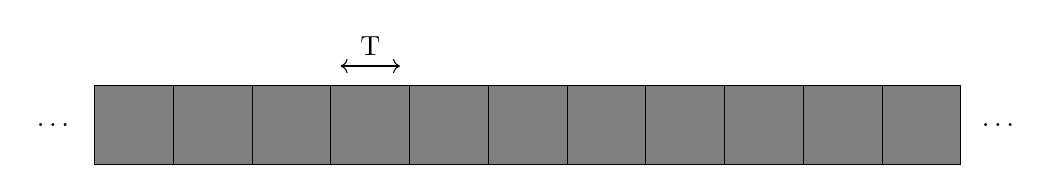
\begin{tikzpicture}

\draw [fill=gray]  (-2,0) rectangle (-1,-1);
\draw [fill=gray]  (-1,0) rectangle (0,-1);
\draw [fill=gray]  (0,0) rectangle (1,-1);
\draw [fill=gray]  (1,0) rectangle (2,-1);
\draw [fill=gray]  (2,0) rectangle (3,-1);
\draw [fill=gray]  (3,0) rectangle (4,-1);
\draw [fill=gray]  (4,0) rectangle (5,-1);
\draw [fill=gray]  (5,0) rectangle (6,-1);
\draw [fill=gray]  (6,0) rectangle (7,-1);
\draw [fill=gray]  (7,0) rectangle (8,-1);
\draw [fill=gray]  (8,0) rectangle (9,-1);

\node (v1) at (-2.5,-.5) {};
\node (v2) at (9.5,-.5) {};
\draw  (v1) node {\dots} ;
\draw  (v2) node {\dots} ;

\node (v3) at (1,.25) {};
\node (v4) at (2,.25) {};
\draw  [<->] (v3) edge (v4);

\node (v5) at (1.5,.5) {};
\draw  (v5) node {T} ;
\end{tikzpicture}
\caption{Uniform sampling with sample period T. Gray blocks are sampled}\label{tkz:uniform}
\end{figure}

When one desires to ensure full reconstruction of the signal with uniform sampling one needs to sample at the Nyquist rate \todo{ref}. To improve our sampling methods we remove the restriction of uniform sampling to look for more efficient ways to sample the spectrum. Non uniform sampling has no restriction on delays of subsequent samples. This is illustrated in \cref{tkz:nonuniform}.

\begin{figure}[H]
\centering
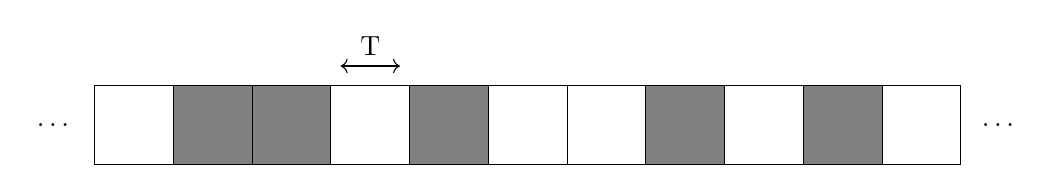
\begin{tikzpicture}

\draw  (-2,0) rectangle (-1,-1);
\draw [fill=gray]  (-1,0) rectangle (0,-1);
\draw [fill=gray]  (0,0) rectangle (1,-1);
\draw  (1,0) rectangle (2,-1);
\draw [fill=gray] (2,0) rectangle (3,-1);
\draw  (3,0) rectangle (4,-1);
\draw  (4,0) rectangle (5,-1);
\draw [fill=gray]  (5,0) rectangle (6,-1);
\draw  (6,0) rectangle (7,-1);
\draw  [fill=gray] (7,0) rectangle (8,-1);
\draw  (8,0) rectangle (9,-1);

\node (v1) at (-2.5,-.5) {};
\node (v2) at (9.5,-.5) {};
\draw  (v1) node {\dots} ;
\draw  (v2) node {\dots} ;

\node (v3) at (1,.25) {};
\node (v4) at (2,.25) {};
\draw  [<->] (v3) edge (v4);

\node (v5) at (1.5,.5) {};
\draw  (v5) node {T} ;
\end{tikzpicture}
\caption{Non-uniform sampling with sample period T. Gray blocks are sampled}\label{tkz:nonuniform}
\end{figure} 

This is however not trivial to implement on a device. To perform non-uniform sampling we introduce multi-coset sampling. Multi-coset sampling is a set of sampling methods that use multiple samplers, or cosets, to sample the spectrum. This is illustrated in \cref{tkz:multicoset}

\begin{figure}[H]
\centering
\begin{tikzpicture}
\draw  (-2.5,2) rectangle (-1.5,1) node[pos=.5]{$x$};
\draw  (-1.5,1.5) -- (0.5,1.5);
\draw  (-0.5,3) -- (0.5,3);
\draw (-0.5,3) -- (-0.5,-0.5);

\node at (2.5,-.91) {\vdots};
\node at (0.75,-.91) {\vdots};
\node at (-0.5,-.91) {\vdots};

\draw (-0.5,-1.5) -- (-0.5,-2);
\draw  (1,3) -- (2,3);
\draw  (1,1.5) -- (2,1.5);
\draw  (1,0) -- (2,0);
\draw  (1,-2) -- (2,-2);
\draw (-0.5,0) -- (0.5,0);
\draw (-0.5,-2) -- (0.5,-2);
\draw[ very thick](0.5,3)-- +(30:0.46);
\draw[ very thick](0.5,1.5)-- +(30:0.46);
\draw[ very thick](0.5,0)-- +(30:0.46);
\draw[ very thick](0.5,-2)-- +(30:0.46);
\draw  (3,2) rectangle (2,1) node[pos=.5]{$y_1$};
\draw  (3,0.5) rectangle (2,-0.5) node[pos=.5]{$y_2$};
\draw  (3,-1.5) rectangle (2,-2.5) node[pos=.5]{$y_m$};
\draw  (3,3.5) rectangle (2,2.5) node[pos=.5]{$y_0$};
\end{tikzpicture}
\caption{schematic multi-coset sampling with $m$ cosets}\label{tkz:multicoset}
\end{figure}

In the reconstruction section we will deduce criteriums on the sampling that will further specify the samplers. In the sampling section methods we will then get back to multi-coset sampling to link it to the reconstruction and optimize performance.

\end{document}

